%! Author = charon
%! Date = 2/8/24

\subsection{Einführung in AFL}\label{subsec:afl}
\gls{afl} ist ein Werkzeug zur automatisierten Programmprüfung.
Es wurde 2013 von Michal Zalewski entwickelt und basiert ursprünglich auf dem Ansatz des Sourcecode-guided Fuzzing.
Dieser Ansatz schreibt vor, dass auf jeden bedingten Sprung, wie beispielsweise einer if-Anweisung in vielen Hochsprachen
wie C oder Java, geachtet wird.
Ein solcher Verzweigungspunkt, an dem der Zustand des Programms verändert werden kann, wird als \textit{basic block} bezeichnet.
\begin{figure}[h]
    \frame{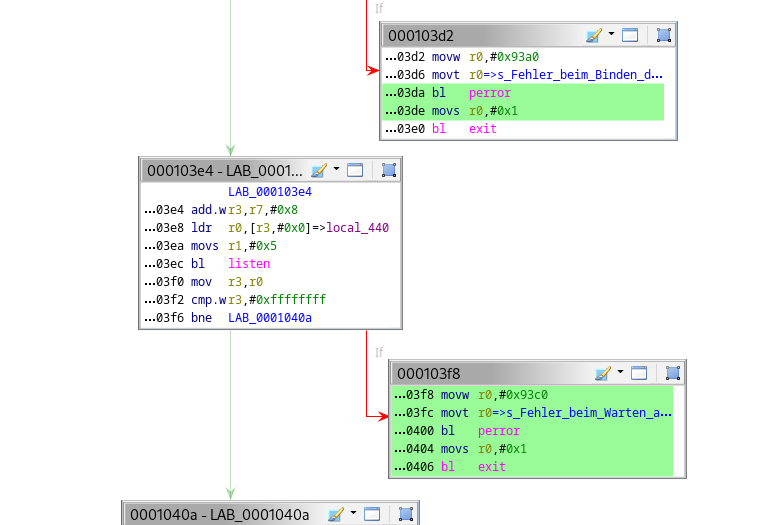
\includegraphics[width=\linewidth]{img/basic-blocks-example}}
    \caption{Zeigt ein Beispiel mehrerer basic blocks. Der hier gezeigte Disassembly und der damit verbundene
    Kontrollflussgraph entstammt dem selbst implementierten \gls{tcp}-Servers aus dem Kapitel \ref{subsubsec:persistent-mode}.
    Verwendet wurde hierbei das Reverse-Engineering-Tool Ghidra.}\label{fig:basic-block}
\end{figure}\\
Ein basic block ist dadurch gekennzeichnet, dass die erste Instruktion als Einstiegspunkt (\textit{entry point}) und die letzte Instruktion
als Ausstiegspunkt (\textit{exit point}) bezeichnet wird.
Ein entry point ist in der Regel die erste Instruktion nach einem Sprung im Codesegment.
Der exit point kann das Ende des Codes oder eine Sprunginstruktion im Codesegment sein.
Die Verbindung zweier basic blocks (in Abbildung~\ref{fig:basic-block} mit Pfeilen dargestellt) wird als \textit{branch edge} bezeichnet.
in dieser Arbeit wird ein Pfad von mehreren miteinander verbundenen basic blocks als Codepfad bezeichnet. \\
\linebreak
Der Programmcode wird klassischerweise zuerst mit dem von \gls{afl} bereitgestellten custom compiler \texttt{afl-cc} kompiliert.
In diesem Schritt wird das Programm von \gls{afl} auf bedingte Sprünge untersucht und an jeder Instruktion wird eigener
Programmcode an diesen Stellen injiziert.
Anschließend wird der dabei entstandene Programmcode kompiliert und ist somit für die Fuzzing-Kampagne vorbereitet. \\
\linebreak\linebreak
Zur Optimierung der Fuzzing-Kampagne kann der Korpus nach dem ersten Durchlauf mit einem weiteren Tool von \gls{afl}
(\texttt{afl-cmin}) minimiert werden.
Bei der Minimierung des Korpus wird darauf geachtet, ob beim Ausführen des Programms neue Programmpfade traversiert werden.
Danach wird die Fuzzing-Kampagne mit dem Tool \texttt{afl-fuzz} gestartet.
Dabei werden in einem Testdurchlauf zuerst alle gesammelten Inputs auf ihre Validität geprüft, indem \gls{afl} darauf
achtet, ob das zu untersuchende Programm in einen definierten Zustand gelangt und fehlerfrei terminiert.
Zusätzlich wird geprüft, welche Programmpfade abgelaufen werden und ob Testfälle neue Programmpfade erreichen.
Diese Strategie bezeichnet man als covered-based Strategie~\cite[vgl.][7]{iot-fuzzing}.\\
\linebreak
Nachdem alle Testfälle erfolgreich durchgeführt wurden, beginnt die Mutation des Inputs.
Hierzu gibt es auch verschiedene Ansätze, die von Fuzzern verfolgt werden.\\
Ein elementarer Bestandteil des \gls{afl} ist der darin enthaltene Forkserver.
Dieser ist für die Vorbereitung des Binaries für die Fuzzing-Kampagne verantwortlich.
Das Binary durchläuft den Syscall \texttt{execve()} einmalig, welcher dafür verantwortlich ist, das zu startende Programm in
den aktuellen Prozess zu laden.
Zudem ist der Forkserver dafür verantwortlich sicherzustellen, dass das zu instrumentierende Programm nur ein Mal
zum Ausführen gelinkt wird und ein Einsprungspunkt für den Fuzzer nach der Initialisierung gesetzt wird.
An diesem Einsprungspunkt werden nach der Initialisierung die Instruktionen -- oder auch Testcases -- der Fuzzing Kampagne von \gls{afl}
injiziert.
Dadurch wird die Performance verbessert, da das Programm bei mehrfacher Ausführung nur jeweils ein Mal initialisiert wird
und der ursprüngliche Zustand des Prozesses wiederhergestellt wird.
Anschließend werden Kopien des Prozesses an der Stelle des Forkservers mithilfe des \texttt{fork()} Syscalls erstellt.
Daher stammt auch der Name Forkserver.
Er setzt einen Startpunkt für den Fuzzer fest, an dem der Prozess des Programms in dem zu der Zeit feststehenden Zustand
mithilfe des \texttt{fork()} Syscalls kopiert wird.
Dieser Prozess wird auch \textit{Forken} genannt.
Dabei entsteht eine logische Einteilung der beiden Prozesse wobei der Elternprozess der Prozess ist, welcher vor dem Forken
bereits vorhanden war.
Der aus dem Forken entstandene Prozess heißt Kindprozess.\\
\linebreak
Die von \gls{afl} genutzte Syntax besteht aus drei Komponenten.
%! Author = chaorn
%! Date = 17.02.24

\begin{lstlisting}[language=bash, caption={Syntax des AFL Fuzzing-Befehls},label={lst:afl-synthax}]
$ afl-fuzz -i in/ -o out/ -- /app/mmapp @@
\end{lstlisting}
Man beginnt mit dem Tool \texttt{afl-fuzz}.
Daraufhin wird das Flag \texttt{-i} mit dem Pfad zum Ordner (hier~\ref{lst:afl-synthax}: \textit{in/}) gesetzt, der den Korpus enthält.
Anschließend daran wird das Flag \texttt{-o} mit dem Pfad zu dem Ordner (hier~\ref{lst:afl-synthax}: \textit{out/}) gesetzt,
in dem die zur Laufzeit der Fuzzing-Kampagne generierten Ergebnisse abgelegt werden.
Zur besseren Lesbarkeit kann nach dem letzten Ordner ein \textit{- -} angefügt werden.
Danach wird der Pfad zur zu untersuchenden Applikation angegeben.
Zuletzt wird die Art der Übermittlung des Inputs dem Binary beschrieben.
Die Zeichen \texttt{@@} stehen für die Kommunikation mit dem Binary mit Dateien.
Die Zeichen dienen als Platzhalter für \gls{aflpp} und werden zur Laufzeit des Fuzzers mit den generierten Daten mit dem
Namen \textit{.curr\_input} ersetzt ~\cite{afl-file-extension}.
Dadurch werden ganze Dateien an das zu untersuchende Binary übergeben.
Wenn man jedoch das \texttt{@@} weglässt, so wird der Inhalt der im Input-Verzeichnis enthaltenen Dateien sequentiell an
das Binary über stdin übergeben. \\
\linebreak
In dieser Arbeit wird ausschließlich \gls{aflpp} verwendet.
\gls{aflpp} ist eine Abzweigung von \gls{afl} und wird von einer breiten Community erweitert und verbessert.
\gls{afl} und \gls{aflpp} unterscheiden sich maßgeblich in der Effizienz der Mutation, der Entdeckung von Codepfaden und
einigen in \gls{afl} nicht umgesetzten Features.
Zur VereinfachungIn wird in den folgenden Kapiteln nur von \gls{afl} als Abkürzung für \gls{aflpp} gesprochen.